\subsubsection{Hilbert Space}

In short, Hilbert Space is a complete inner-product space that is infinite-dimesional.

\begin{mystthmdefinition}{Hilbert Space}{definition-hilbertspace-1}Let $X$ be a complex vector space. An \textbf{inner product} is a function from $X \times X \to \mathbb{C}$
\begin{equation}
(x,y)\mapsto \langle x,y \rangle
\end{equation}
if it satisfies, $\forall x,y, z \in X$

\begin{enumerate}
\item $\langle ax+by, z\rangle=a\langle x,z \rangle + b\langle y, z\rangle$
\item $\langle x,y \rangle = \overline{\langle y, x\rangle}$
\item $(x,z)\in (0,\infty)$
\end{enumerate}

The pair $(X,\langle \cdot, \cdot\rangle)$ is a \textbf{pre-Hilbert space}. It is also a Banach Space with norm induced by the inner product:
\begin{equation}
\|\cdot \| = \langle\cdot, \cdot \rangle^{1/q}
\end{equation}
If $X$ is also complete, it is a \textbf{Hilbert Space}

\end{mystthmdefinition}
\paragraph{The Riez Representation Theorem}

\begin{mystthmtheorem}{Riez Representation Theorem}{theorem-hilbertspace-2}Let $f\in H^*$, $\exists !$ $y\in H$ such that $\forall x\in H$ we have:
\begin{equation}
f(x)=\langle x,y \rangle
\end{equation}

\end{mystthmtheorem}
\paragraph{The Basis Theorem}

\begin{mystthmtheorem}{Bessel's Inequality}{theorem-hilbertspace-3}If $\{u_{\alpha}\}_{\alpha \in A}$ is an orthonormal set in $H$, then for any $x\in H$:
\begin{equation}
\sum_{\alpha \in A}|\langle x, u_{\alpha}\rangle|^2 \leq \|x\|^2
\end{equation}
Note this implies $\{\alpha: \langle x,u_{\alpha} \rangle\neq 0\}$ is countable

\end{mystthmtheorem}
\begin{mystthmtheorem}{Basis Theorem}{theorem-hilbertspace-4}If $\{u_{\alpha}\}_{\alpha \in A}$ is an orthonormal set then the following are equivalent:

\begin{enumerate}
\item (\textit{Completeness}) If $\langle x,u_{\alpha}\rangle =0, \forall \alpha \in A$ then $x=0$
\item (\textit{Parseval's Identity}) $\forall x\in H$

\begin{equation}
\|x\|^2 = \sum_{\alpha \in A} |\langle x, u_{\alpha} \rangle|^2
\end{equation}


\item (\textit{Representation}) $\forall x\in H$

\begin{equation}
x = \sum_{\alpha \in A} \langle x, u_{\alpha} \rangle u_{\alpha}
\end{equation}
\end{enumerate}

\end{mystthmtheorem}
\begin{mystthmproof}{}{proof-hilbertspace-5}$(1)\Longrightarrow (3)$ Let $x\in H$, let $\{\alpha_j\}$ be a enumeartion of nonzero terms in the sum $\sum_{\alpha \in A} \langle x, u_{\alpha} \rangle u_{\alpha}$
\begin{equation}
\sum_{j=1}^{\infty} \langle x, u_{\alpha_j}\rangle u_{\alpha_j}=\sum_{\alpha \in A} \langle x, u_{\alpha}\rangle u_{\alpha}
\end{equation}
Using orthonormality we have\footnote{This is often referred to as the \textit{Pythagorean's Theorem}, stating that for mutually orthogonal vectors$\{a_j\}_{j=1}^{\infty}$:
\begin{equation}
\|\sum_j a_j\|^2 = \sum_{a_j}\|a_j\|
\end{equation}
In particular, if we take only two vectors $a \perp b \in \mathbb{R}^2$, this becomes the Pythagorean's Theorem in middle school:
\begin{equation}
\|a\|^2 + \|b\|^2 = \|c\|^2
\end{equation}}:
\begin{equation}
\begin{aligned}
\left \| \sum_{n}^m \langle x, u_{\alpha_j} \rangle u_{\alpha_j} \right \|^2 &= \left\langle \sum_{n}^m  \langle x, u_{\alpha_j} \rangle u_{\alpha_j}, \sum_{n}^m  \langle x, u_{\alpha_k} \rangle u_{\alpha_k} \right\rangle  \\
&= \sum_{n}^m \left| \langle x, u_{\alpha_k} \rangle \right|^2
\end{aligned}
\end{equation}
By Bessel's inequality, we know $\sum_{j}\left| \langle x, u_{\alpha_j} \rangle \right|^2$ converges. This implies\footnote{Suppose we are confronted by the series  $s=\sum_{1}^{\infty}a_j$ which converges absolutely to $L$.
Need: given $\epsilon>0$, there exists $N(\epsilon)$ such that $\forall N<n<m$ we have $\sum_{n}^m |a_j| < \epsilon$.
We can pick $N$ such that $\left|\sum_{j=1}^k |a_j| -L\right| < \epsilon/2$, $\forall k\geq N$. But now forall $m>n>N$, we have:
\begin{equation}
\begin{aligned}
\sum_{n}^m |a_j| &= \sum_{1}^m |a_j| - \sum_1^{n-1} |a_j|   \\
\end{aligned}
\end{equation}} the tail can be made arbitarily small, i.e., $\forall \epsilon >0$, {\textbackslash}exists $N(\epsilon)$ such that $\forall N<n<m$ we have:
\begin{equation}
\sum_{n}^m \left| \langle x, u_{\alpha_k} \rangle \right|^2  < \epsilon
\end{equation}

\end{mystthmproof}
\paragraph{The Sturm-Liouville Operator}

The \textbf{Sturm-Liouville operator} is a linear differential operator of the form
\begin{equation}
\mathcal L=-\frac{d}{dx}\left(p\frac{d}{dx}y\right)+q\frac{d}{dx}
\end{equation}

We've shown that the Sturm-Liouville opeartor is self-adjoint with appropriate boundary condition in the sense that:
\begin{equation}
\begin{aligned}
\langle u, \mathcal Lv \rangle &= \langle \mathcal L^*u, v \rangle
\end{aligned}
\end{equation}
hence it is analgous to self-adjoint operator in finite-dimensional vector spaces, which as symmetric matrix representation when the underlying field is real. We now make this connection explicit, i.e., actually constructing the discretized, finite-dimensional matrix representation of the Sturm-Liouville Operator.

\subparagraph{A Discrete Analog}

Let's consider a concrete SL opeartor defined on $[0,1]$ with Dirchlet boundary condition $y(0)=y(1)=0$. Instead of directly discretizing $\mathcal L$, we aim to find a matrix $L$ such that discretizes the quadratic form:
\begin{equation}
F(y)=\int y\mathcal Ly dx \rightarrow \hat y^TL\hat y
\end{equation}
First we note that:
\begin{equation}
\label{func}
\begin{aligned}
F(y) &= \int_0^1 y\left(-\frac{d}{dx}\left(p\frac{d}{dx}y\right) + qy\right) dx \\
&= \int_0^1 -y \frac{d}{dx}\left(p\frac{d}{dx}y\right)dx+\int_0^1 qy^2dx  \\
&= -\left\{\cancel{\left[yp\frac{dy}{dx}\right]_0^1} - \int p\left(\frac{dy}{dx}\right)^2 \right\} + \int_0^1 qy^2dx \\
&= \int_0^1 py'^2 + qy^2
\end{aligned}
\end{equation}
Now we discretize $y, p, q$ to $N$-dimensional arrays:
\begin{equation}
\begin{aligned}
\hat y &= [y_1,...,y_N] \\
\hat p &= [p_1,...,p_N] \\
\hat q &= [q_1,...,q_N]
\end{aligned}
\end{equation}
Using forward difference we get:
\begin{equation}
\hat y =\left(\frac{y_{i+1}-y_i}{h}\right)^2
\end{equation}
Rewrite the integral as a finite sum we obtain a discretized version of (\ref{func}):
\begin{equation}
\boxed{\hat F(\hat y)=\sum_{i=1}^N h p_i\left(\frac{y_{i+1}-y_i}{h}\right)^2 +q_iy_i^2}
\end{equation}
Our goal is now to find a matrix $L$ such that $\hat y^TL\hat y=\hat F(\hat y)$. Rewrite $\hat F(\hat y)$:
\begin{equation}
\hat F(\hat y) =\sum_{i=1}^N Np_i(y_{i+1}^2 -2y_{i+1}y_i +y_i^2)+\frac{1}{N}q_iy_i^2
\end{equation}
We can split $L=L_1+L_2$ such that

\begin{enumerate}
\item $\hat y^T L_1 \hat y = \sum_{i=1}^N Np_i(y_{i+1}^2 -2y_{i+1}y_i +y_i^2)$
\item $\hat y^T L_2 \hat y = \sum_{i=1}^N \frac{1}{N}q_iy_i^2$.
\end{enumerate}

\textbf{(Constructing $L_1$)}
Let's first deal with $L_1$. Consider the $2\times 2$block with the upperleft corner at $(i,i)$ that should
represent $Np_i(y_{i+1}^2 -2y_{i+1}y_i +y_i^2)$. This is easy:
\begin{equation}
\begin{aligned}
A_i=Np_i\begin{pmatrix}
1 & -1\\
-1 & 1 \\
\end{pmatrix}
\end{aligned}
\end{equation}
To assemble $L_1$ we can overlap $A_i$ along the diagonal of $L$ with a stride of 1. Concretely:

\begin{mystcodebox}
\begin{verbatim}
for i=1,...,N -1
    L[i,i] += Np_i
    L[i+1,i+1] += Np_i
    L[i,i+1] -= Np_i 
    L[i+1,i] -= Np_i
\end{verbatim}

\end{mystcodebox}
\begin{mystthmexample}{}{example-hilbertspace-6}A quick example for $N=4$:
\begin{equation}
\begin{aligned}
4\begin{pmatrix}
p_1 & -p_1 & 0 & 0 \\
-p_1 & p_1+p_2 & -p_2 &0 \\
0 & -p_2 & p_2+p_3 & -p_3 \\
0 &  0 & -p_3  & p_3
\end{pmatrix}
\end{aligned}
\end{equation}

\end{mystthmexample}
\textbf{(Constructing $L_2$)}
$L_2$ is purely diagonal and is easier to derive. Since it only has quadratic term $y_i^2$, at each row $i$ we only need to include $y_i$. Hence:
\begin{equation}
\begin{aligned}
L_2 = \frac{1}{N}\begin{pmatrix}q_1 & & \\
& \ddots & \\
& & q_N
\end{pmatrix}
\end{aligned}
\end{equation}

\textbf{(Assembly $L_1+L_2$)}
It is clear that $L$ should look like:

\begin{equation}
\begin{aligned}
L=N\begin{pmatrix}
p_1&  -p_1 & & &  \\
-p_1& p_1+p_2 &  -p_2 & &  \\
&  \ddots  &  \ddots &   \ddots &   \\
&  &-p_{N-1} &p_{N-1}+p_{N} & -p_N  \\
& & &-p_N & p_N \\
\end{pmatrix} 
+ 
\frac{1}{N}\begin{pmatrix}q_1 & & \\
& \ddots & \\
& & q_N
\end{pmatrix}
\end{aligned}
\end{equation}

However, since we are dealing with concrete operators with accompanying domain and boundary condition, we need to encoorperate the Dirchelt boundary condition $y(0)=1, y(1)=0$ into $L$. To do so we need to zero-out the first row and column of $L$. Hence finally we get:

\begin{mystthmproposition}{}{proposition-hilbertspace-7}The Sturm-Liouville Operator on $[0,1]$ with Dirchlet boundary condition $y(0)=y(1)$ can be discretized as
\begin{equation}
\label{discretesl}
\begin{aligned}
L=N\begin{pmatrix}
0 &0 & & &  &\\
0 &p_1+p_2 & -p_2& & & \\
&-p_2&  \ddots &\ddots & -p_{N-1}& \\
& & \ddots &-p_{N-1} & p_{N-1}+p_N &0 \\
& & & &0 & 0\\
\end{pmatrix} 
+ 
\frac{1}{N}\begin{pmatrix}0 & & & & \\
& q_2 & & & \\
&  & \ddots& & \\
& & & q_{N-1} & \\
& &  & & 0  \\
\end{pmatrix}
\end{aligned}
\end{equation}

\end{mystthmproposition}
We can see that $L$ is indeed a symmetric real matrix(Hermitian)!

\textbf{Numpy Implementation}
This can easily be translated to naive \texttt{numpy} code:

\begin{mystcodebox}
\begin{verbatim}
class SturmLiouville:
    def __init__(self,N, p, q=None, grid='forward'):
        A = np.zeros(shape=(N,N))
        if grid == 'forward':
            for i in range(N -1):
                A[i, i] += p[i]
                A[i+1, i+1] += p[i]
                A[i, i+1] -= p[i]
                A[i+1, i] -= p[i]

        if q is not None:
            I = np.eye(N) 
            L = A + q @ I
        else:
            L = A
        
        # Dirchlet Boundary Condition
            L[0,0]=0.0
            L[0,1]=0.0
            L[1,0]=0.0
            L[N -1,N -1]=0.0
            L[N -1,N -2]=0.0
            L[N -2,N -1]=0.0
        self.L = (L * N ** 2)
        self.N = N

    def solve_eigen(self, top_k=10):
        eval, evec = np.linalg.eig(self.L)
        top_k_idx = np.argsort(eval[eval>0])[:top_k]
        return eval[top_k_idx] , evec[:, top_k_idx], top_k_idx
\end{verbatim}

\end{mystcodebox}
\textbf{Example: $-\frac{d^2}{dx^2}$ as a Matrix}
We can do a quick example to showcase that $L$ is indeed a discretization of $\mathcal L$.

\begin{mystthmexample}{-$\frac{d^2}{dx^2}$}{example-hilbertspace-8}We have already seen that the opeartor:
\begin{equation}
T=-\frac{d^2}{dx^2}, D(T)=\{y,Ty \in L^2[0,1]:y(0)=y(1)=0\}
\end{equation}
has eigenvalues and eigenvectors:
\begin{equation}
\begin{aligned}
y_j(x) &=\sqrt{2}\sin j\pi x \\
\lambda_j &= j^2\pi^2
\end{aligned}
\end{equation}
for $j=1,2,3...$. The problem is that, can we solve a matrix eigenvalue problem to recover exactly the same result?
Indeed we can! Passing $p= -1$ and $q=0$ gets us:
\begin{equation}
\begin{aligned}
L=N\begin{pmatrix}
0 & 0 & &  &  \\
0 & 2 & -1 & &  \\
 & -1 & \ddots & \ddots & \\
& & \ddots & 2 & -1  &\\
& & & -1& 2 & 0\\
& & & & 0 & 0 \\
\end{pmatrix}
\end{aligned}
\end{equation}

and solving the matrix eigenvalue problem
\begin{equation}
\begin{aligned}
L\hat y &= \lambda \hat y
\end{aligned}
\end{equation}
 gets us:
\footnote{Since iterative eigensolvers gives eigenvectors of arbitrary magnitude $v_j=a\sin(j\pi(x))$, we need to normalize properly by
1.Ensure $a>0$

\begin{enumerate}
\item Divide by $\sqrt{\sum y_i^2 h}$
\end{enumerate}}

\end{mystthmexample}
\begin{figure}[!htbp]
\centering
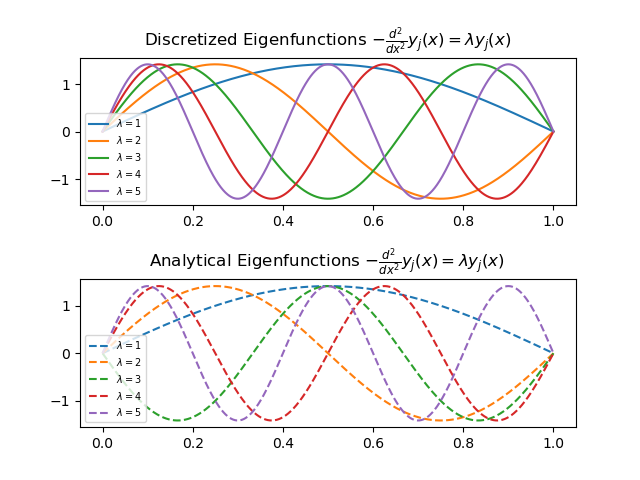
\includegraphics[width=0.7\linewidth]{files/sl_evecs-749bd46b634f4b726002411b1a849030.png}
\end{figure}

\begin{mystexercise}{}{exercise-e5eisbchmw}\label{exercise-E5EisbCHMW}\label{exercise-e5eisbchmw}\begin{enumerate}
\item We discretized $L$ based on the quadratic form $\int_0^1 y\mathcal L y dx$, hence $\hat y^T L\hat y$ should coincide with $\int_0^1 y\mathcal L y dx$. Come up with at least 2 functions and 2 operators that satisfy the requirment($L^2(0,1),y(0)=y(1)=0$). Compute the quadratic form analytically and numericaly. Cheeck that the results are the same.
\item Remove the masking code snippet(which implements Dirchlet boundary condition) in the naive SL class \texttt{SturmLiouville}. What is the resulting eigenvectors? Explain the result.
\item Try coming up with different discretization with center difference or back difference. Implemet it in \texttt{python}
or \texttt{julia}.

\begin{itemize}
\item Is the resulting matrix $L$ still symmetric ?
\item Center differencing scheme results in a numerical artifcat, what is the numerical artifact? Try explaining why such artifact occur(\textit{Hint: Note that even and oddd indicies are decoupled})
\end{itemize}
\end{enumerate}

\end{mystexercise}
%  
% :::{note} Optimizing $x^TAx$ gives $Ax=\lambda x$
% Let $x\in \mathbb{R}^n$, $A\in \mathbb{R^{n\times n}}$ is a **symmetric** matrix, define:
% $$
% F(x)=\frac12 \langle x,Ax \rangle
% $$
% Consider the optimization of $F$ constrained on $\|x\|^2=1$ 
% :::
% 
% We use lagarange multiplier:
% $$
% (Ax)^T+x^TA-2\lambda x^T &=0 \\
% Ax + A^Tx - 2\lambda x &=0 \\
% 2(A-\lambda I)x&=0 \\
% Ax &= \lambda x
% $$ 
% [^diff]
% Subjected to $\|x\|^2=1$. We note that this is an **eigenvalue problem**. 
%